\section{Evaluation of Transitions}
\label{sec:transition-evaluation}

Helena puts some restrictions on the variables of transitions in order
to be able to efficiently compute enabled transition bindings at a
given marking.  Besides the fact that all variables of a transition
have to be declared by appearing in a tuple labelling its input or
inhibitor arcs or otherwise in the pick section, additional
constraints are put on these variables.  We summarize below the
evaluation process in two situations: when the transition does not
have inhibitor arcs and when it does.

\subsection{Evaluation in the absence of inhibitor arcs}
During the computation of the enabled bindings of a transition that
does not have any inhibitor arc, Helena has to evaluate the labels of
the input arcs of the transition, its guard, and finally has to pick
all the possible acceptable values for its free variables defined in
the pick section.  Hence, three types of items have to be evaluated to
bind all the variables of the transition and find enabled bindings:
tuples of input arcs, the guard, and free variables.

Each of these items define some variables, i.e., bind them by giving
them a value, and use some variables that have to be defined so that
the item can be evaluated.  The table below summarizes which variables
are used/defined by each kind of item.

\begin{center}
\begin{tabular}{|c|c|c|}
\hline
Item & Variables used & Variables defined\\
\hhline{===}
Tuple
& all variables appearing in the tuple
& all variables appearing in the tuple\\
& (and not defined in it)
& at the top level (not in a sub-expression)\\
\hline
Guard & all variables appearing in the guard & none\\
\hline
Free variable
& all variables appearing in the definition of the variable
& the variable\\
\hline
\end{tabular}
\end{center}

In the absence of inhibitor arcs a transition must fulfill the
following requirement to be firable: there must be an evaluation order
$item_1$,\ldots,$item_n$ such that, for any $i \in \{1..n\}$ and any
variable $v$ used by $item_i$, there is $j \in \{1..i-1\}$ such that
$item_j$ defines variable $v$.  Otherwise, the transition will not be
evaluable.  This is for example the case with transitions
\lstinline{t} and \lstinline{u} defined below:

\begin{lstlisting}
transition t {
   in  { p: <(x, f(y))> + <(y, x * 2)>; }
   out { q: <(x)>; }
}
transition u {
   in  { p: <(x, f(y))>; }
   out { q: <(x)>; }
   pick { y in g(x); }  //  g returns a set of integers
}
\end{lstlisting}

For transition \lstinline{t} the tuple \lstinline{<(x, f(y))>} defines
variable \lstinline{x} but to evaluate it we require that
\lstinline{y} must be defined.  The tuple \lstinline{<(y, x * 2)>}
defines this variable but needs itself variable \lstinline{x} to be
defined.  Hence, there is here a cyclic dependency.  We face the same
problem for transition \lstinline{u}.

The invokation of Helena on this example will raise the following
errors:
\begin{verbatim}
test.lna:4: Transition t cannot be evaluated
test.lna:8: Transition u cannot be evaluated
\end{verbatim}

\subsection{Evaluation in the presence of inhibitor arcs}
If the transition has inhibitor arcs then the process described in the
previous section first takes place.  If we have found some binding for
the variables defined in the input tuples or in the pick section of
the transition then a second evaluation process starts for the
inhibitor arcs of the transition.  To be firable, there must not be
any binding for the variables defined by inhibitor arcs such that the
corresponding tokens are present in the place linked by the inhibitor
arc.

Let us for instance consider the following transitions.

\begin{lstlisting}
transition t {
   in      { p: <(x)>; }
   out     { q: <(x)>; }
   inhibit { r: <(x)>; }
}
transition u {
   in      { p: <(x)>; }
   out     { q: <(x)>; }
   inhibit { s: <(x, y)>; }
}
\end{lstlisting}

Transition \LS{t} is firable for some binding \LS{x} if and only if
the token \LS{<(x)>} is present in \LS{p} but not in \LS{r}.
Transition \LS{u} is firable for some binding \LS{x} if and only if
the token \LS{<(x)>} is present in \LS{p} and there exists no \LS{y}
such that the token \LS{<(x, y)>} is present in \LS{s}.

Note that variables defined in inhibitor arcs are not variables of the
transition.  For example, variable \LS{y} of transition \LS{u} serves
only during the evaluation of the transition.

\section{Tips and Tricks}
This section gives some hints to use Helena in an efficient way.


\paragraph{Saving memory}
Helena provides some predefined data types. However, we encourage
users to define application specific data types in order to limit the
possible values of variables, and to save memory when markings are
stored in the reachability set. Let us consider for instance a place
with domain \texttt{int}. Each token of this place will be encoded in
a marking with 32 bits. However, if we know that the tokens of this
place can only belong to the range [0..50], it is preferable to define
a new range type ranging from 0 to 50. Thus tokens will fit in 6 bits
instead of 32. If you are not sure of this range, use option
\longForm{run-time-checks} to detect expressions going out of
range. For the same reason, try to limit capacities of places. Option
\longForm{run-time-checks} will also detect violated capacities.


\paragraph{Storage methods}
We advise to proceed as follows when verifying a property :
\begin{itemize}
\item Use a partial search with hash compaction method (option
  \longForm{hash-compaction}).  This method can explore a large
  portion of the state space and report errors much faster.
\item If no error is found during the first stage, use the default
  storage method without compression technique.
\item If the second search ran out of memory, use compression
  techniques (option \longForm{delta}) and rerun the search.
\end{itemize}


\paragraph{Run time checks}
Enabling run time checks usually slows the analysis since additional
code is put in the generated code to check that no error occurs. When
the net contains many arithmetic operations the run time can grow
significantly. Thus, we advise to disable run time checks if no error
is suspected in the model.


\paragraph{Expressing properties}
Analysis techniques and reductions, i.e., partial order reduction,
performed by Helena depends on the property to be checked.  The
reduction observed decreases with the complexity of the property.
Thus, try to verify properties separately when possible.  For
instance, instead of verifying \lstinline{p and q}, verify first
\lstinline{p} and then \lstinline{q}.


\paragraph{Depth- vs. Breadth-first search}
Depth (option \longForm{algo=DFS}) and breadth-first search (option
\longForm{algo=BFS}) both perform a full state space search.
Depth-first search usually leads to better reduction than
breadth-first search, especially when partial order methods are used
(option \longForm{partial-order}).  Breadth-first search, however,
reports counter examples of minimal length.  Thus, keep in mind these
two factors when choosing the type of search to apply.  Though the
techniques implemented in Helena are fully automatic and do not
require any assistance from the user, some informations can be put in
the specification in order to guide Helena into the search and
optimize some of these techniques. We detail now these features.\\


\section{Guiding Helena in the search}
\label{sec:helping-helena}
Some informations provided by the user are not mandatory but given to
Helena in order to make its search more efficient.  However, Helena
does not have any mean to check the validity of the informations
provided.  Thus if some of these revealed to be erroneous Helena could
produce wrong results, e.g., report that a property is verified
whereas it is not.  We therefore encourage users to be very careful
when supplying these informations and to ignore them if there is any
doubt regarding their validity.

\subsection{Typing places}
A type can be associated to each place of the net. This type specifies
the nature of the information modeled by the place. The types provided
allow to model concurrent systems and protocols synchronizations through
shared variables and communication buffers. Six kinds of places are
allowed: process places, local places, shared places, protected
places, buffer places and ack places.

\begin{figure}[!h]
\begin{center}
\begin{tabular}{cp{0.5cm}c}
\scalebox{0.55}{\input{process.pdf_t}}&~~&
\scalebox{0.55}{\input{local.pdf_t}}\\
A set of cyclic processes &&
Incrementation of the local variable $I$\\
&&\\&&\\
\scalebox{0.55}{\input{shared_protected.pdf_t}}&&
\scalebox{0.55}{\input{buffer_ack.pdf_t}}\\
An incrementation of the shared variable $I$. &&
A synchronous exchange between clients and servers
\\
A lock guarantees exclusive access to $I$.\\&&\\
\multicolumn{3}{c}{\fbox{\scalebox{0.5}{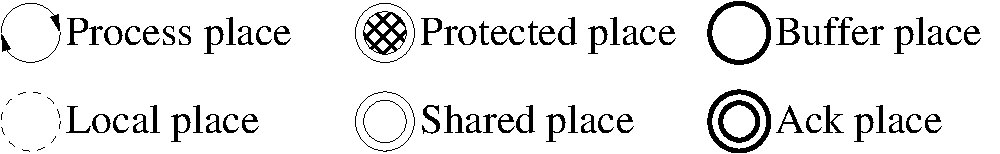
\includegraphics{legend}}}}\\
\multicolumn{3}{c}{Graphical representation of the different place types}\\
\end{tabular}
\end{center}
\caption{Four example nets illustrating the possibility of place typing.}
\label{fig_place_typing}
\end{figure}

\paragraph{Process places (Figure~\ref{fig_place_typing}, top left)}
Process places model the control flow of processes, i.e., its position
in the code it executes. A process is therefore in exactly one of the
process places of the net.  The simple net depicted models cyclic
process.  Each process $p$ can go from state $Idle$ to state
$Working$.  Thus, for each process $p$ there is a token $\tuple{p}$ in
place $Idle$ or in place $Working$.

\paragraph{Local places (Figure~\ref{fig_place_typing}, top right)}
Local places model resources local to a process. Intuitively, this
means that two different processes cannot withdraw the same token from
a local place. The net depicted models the incrementation by 1 of a
local variable $I$. This variable is modeled by the place $I$. The
first component of the domain of this place is the identifier of the
process which owns the local variable and the second one gives the
value of this variable. Since a process $p$ can only access its own
variable and withdraw a token of type $\tuple{p,i}$ from place $I$ we
can type this place as local. Indeed, two different process cannot
currently consume the same token in place $I$.

\paragraph{Shared and protected places (Figure~\ref{fig_place_typing}, bottom left)}
Shared places model resources shared by processes. Shared variables or
locks are examples of informations which can be modeled by a shared
place. Protected places are special shared places. They are used to
model resources which can be accessed by several processes but which
cannot be accessed concurrently thanks to a mechanism, e.g., a mutex,
which guarantees that two processes cannot simultaneously access the
resource.  The net depicted models the incrementation of a shared
variable $I$. To update the value of $I$, a process must first grab a
lock modeled by place $Lock$. This lock ensures that two processes
cannot concurrently update $I$. We can thus declare $I$ as
protected. The place $Lock$ is naturally a shared place since
processes compete for the acquisition of this lock.

\paragraph{Buffer and ack places (Figure~\ref{fig_place_typing}, bottom right)}
Processes can also synchronize themselves by sending messages on
communication channels. These channels are modeled by buffer
places. These places can be thought of as shared places but there is a
major difference between the two: a token residing in a buffer place
can only be removed by a single process. Thus, channels represented by
buffer places are multiple senders - single receiver channels.

Ack places are special kinds of buffer places used to represent
acknowledgments of synchronous exchanges. For instance if process
$p_1$ sends a message to process $p_2$, then waits for the
acknowledgment of $p_2$ before continuing its execution, the place
which corresponds to the acknowledgment can be typed as ack.

The depicted net models the behavior of a set of clients which
interact through messages exchanges. A client $c$ sends a request to a
server $s$ by putting a token $\tuple{c,s}$ in place $Requests$. Since
the only server which can receive this request and withdraw the token
$\tuple{c,s}$ from place $Requests$ is $s$ we can type this place as a
buffer place. Once received by the server the request is treated and
an acknowledgment is sent to the client which can continue its
execution. Since this exchange is a synchronous one, the place $Acks$
can be typed as an ack place.

\subsection{Safe transitions}

\begin{figure}[!h]
\centerline{\scalebox{0.55}{\input{safe.pdf_t}}}
\caption{Transition $Release$ is safe. $Take$ is not.}
\label{fig_safe}
\end{figure}
Transitions of the net can be declared as safe.  A transition binding
is safe if it cannot be disabled by the firing of another binding.  In
other words, the tokens consumed by the binding cannot be stolen by
another binding.  If a transition of the net is declared as safe, then
Helena considers that all the possible bindings of the transition are
safe.

Figure~\ref{fig_safe} depicts an example of safe transition.  Each
process can be in place $Idle$ in place $Working$.  To go to work, a
process must first acquire an object $o$.  The objects are initially
in the place $Objects$.  When a process returns to place $Idle$, it
puts back the object in place $Objects$.  A token $\tuple{p,o}$ in
place $Taken$ means that process $p$ has taken object $o$.

The transition $Take$ is clearly not safe.  Indeed, each enabled
binding $(Take,\tuple{p,o})$ needs a token $o$ in place $Objects$, and
this token can be removed by any other process $q$ which wishes to
acquire the same object.  Thus $(Take,\tuple{q,o})$ disables
$(Take,\tuple{p,o})$.  Let us now have a look at transition $Release$.
Once the binding $(Take,\tuple{p,o})$ is fired, there is a token
$\tuple{p}$ in place $Working$ and a token $\tuple{p,o}$ in place
$Taken$.  Since $p$ is the only process which can remove token
$\tuple{p,o}$ from place $Taken$, the transition binding
$(Release,\tuple{p,o})$ is safe.  This obviously holds for any process
$p$ and object $o$.  Consequently we can declare transition $Release$
as safe.
